\documentclass[11pt]{book}
\usepackage[hidelinks]{hyperref}
\usepackage{float}
\usepackage{graphics}
\usepackage{pdfpages}
\usepackage{graphicx}
\setcounter{tocdepth}{3}
\setcounter{secnumdepth}{3}


\title{Media and Political Imagination}
\begin{document}
\maketitle
\tableofcontents


\part{Lecture Note.}
	\chapter{Week 1.}
		\section{\textcolor{red}{NOTE: NO CLASS.}}

	\chapter{Week 2.}
		\section{\textcolor{red}{NOTE: NO CLASS.}}

	\chapter{Week 3.}
		\section{Day 1; 18 August 2025.}
			\subsection{Class Introduction \& Syllabus.}
				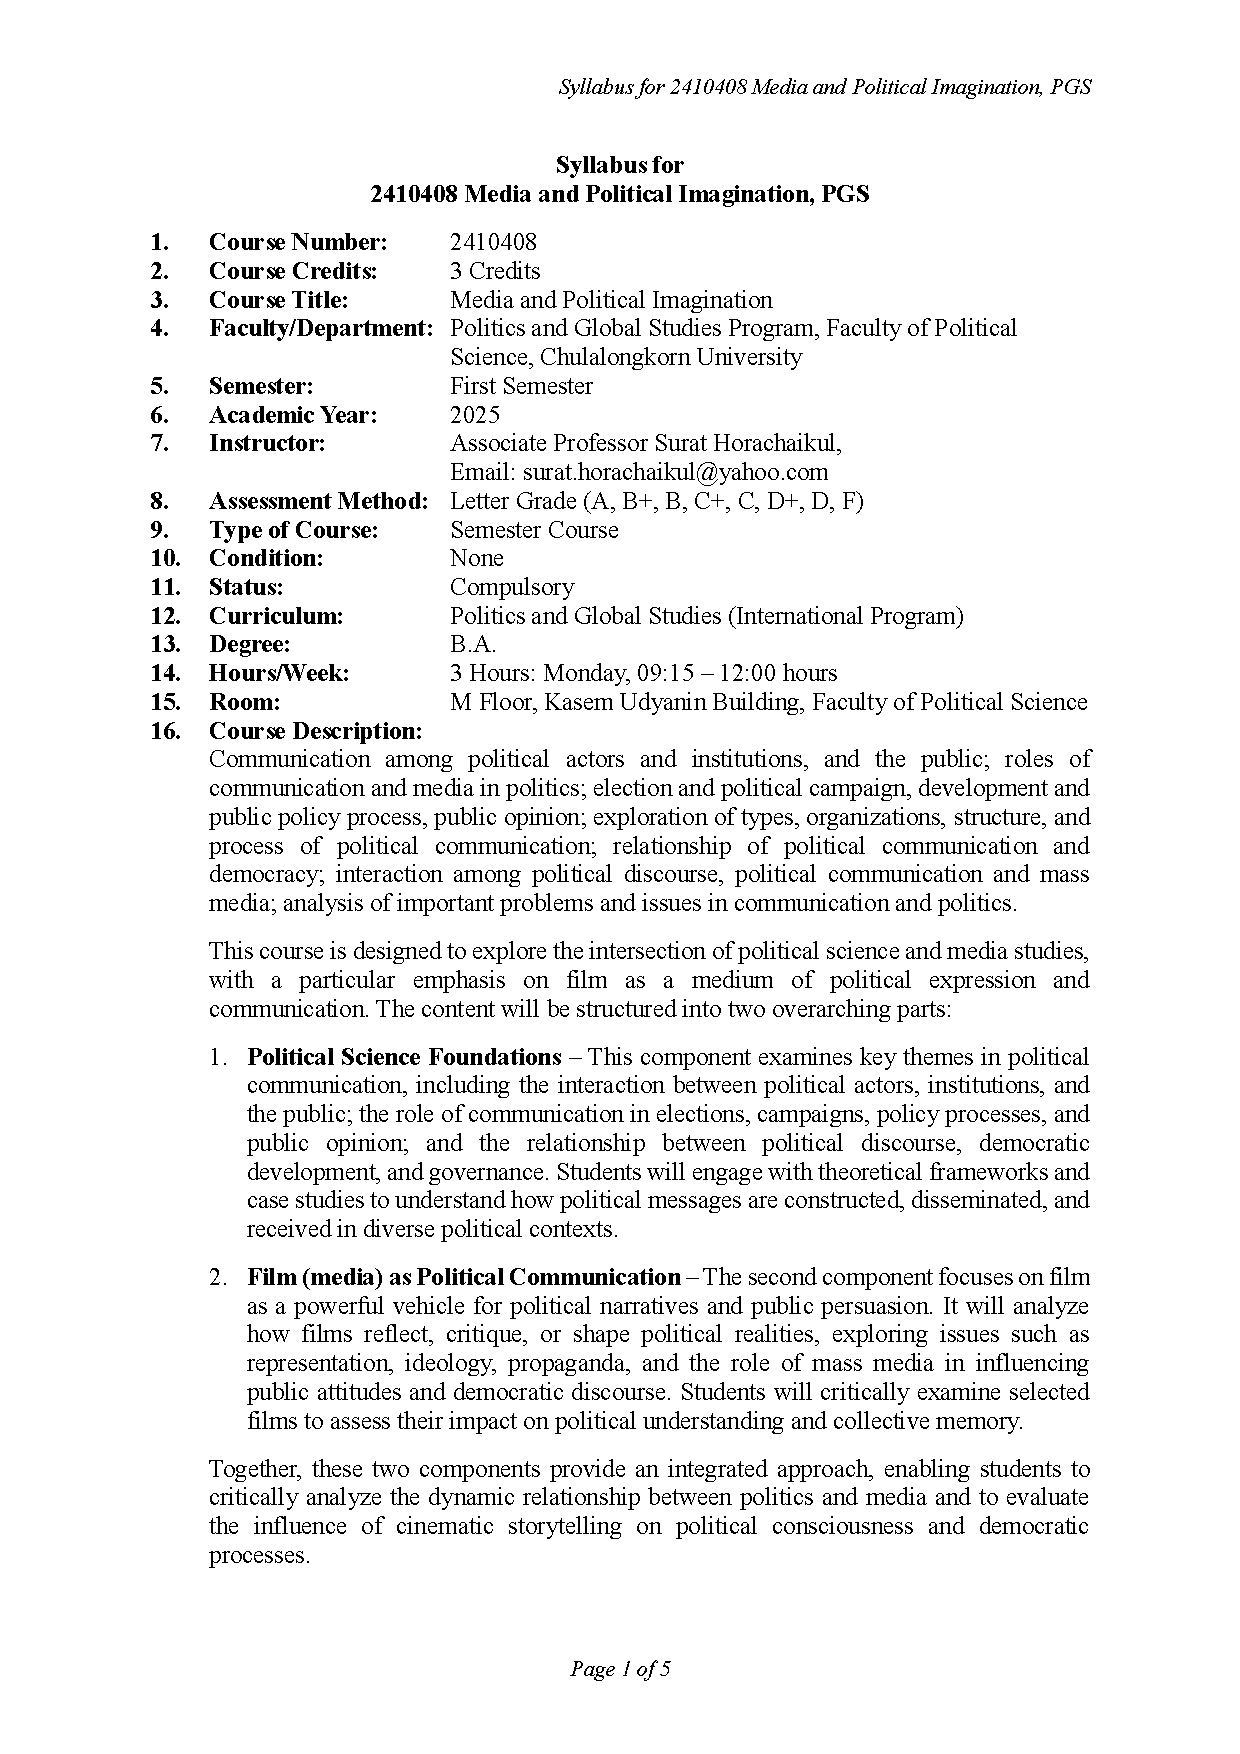
\includepdf[page=-]{Materials/Syllabus_MEDIA_POL_SCI.pdf}
				
			\subsection{Politics, and Political Science.}
				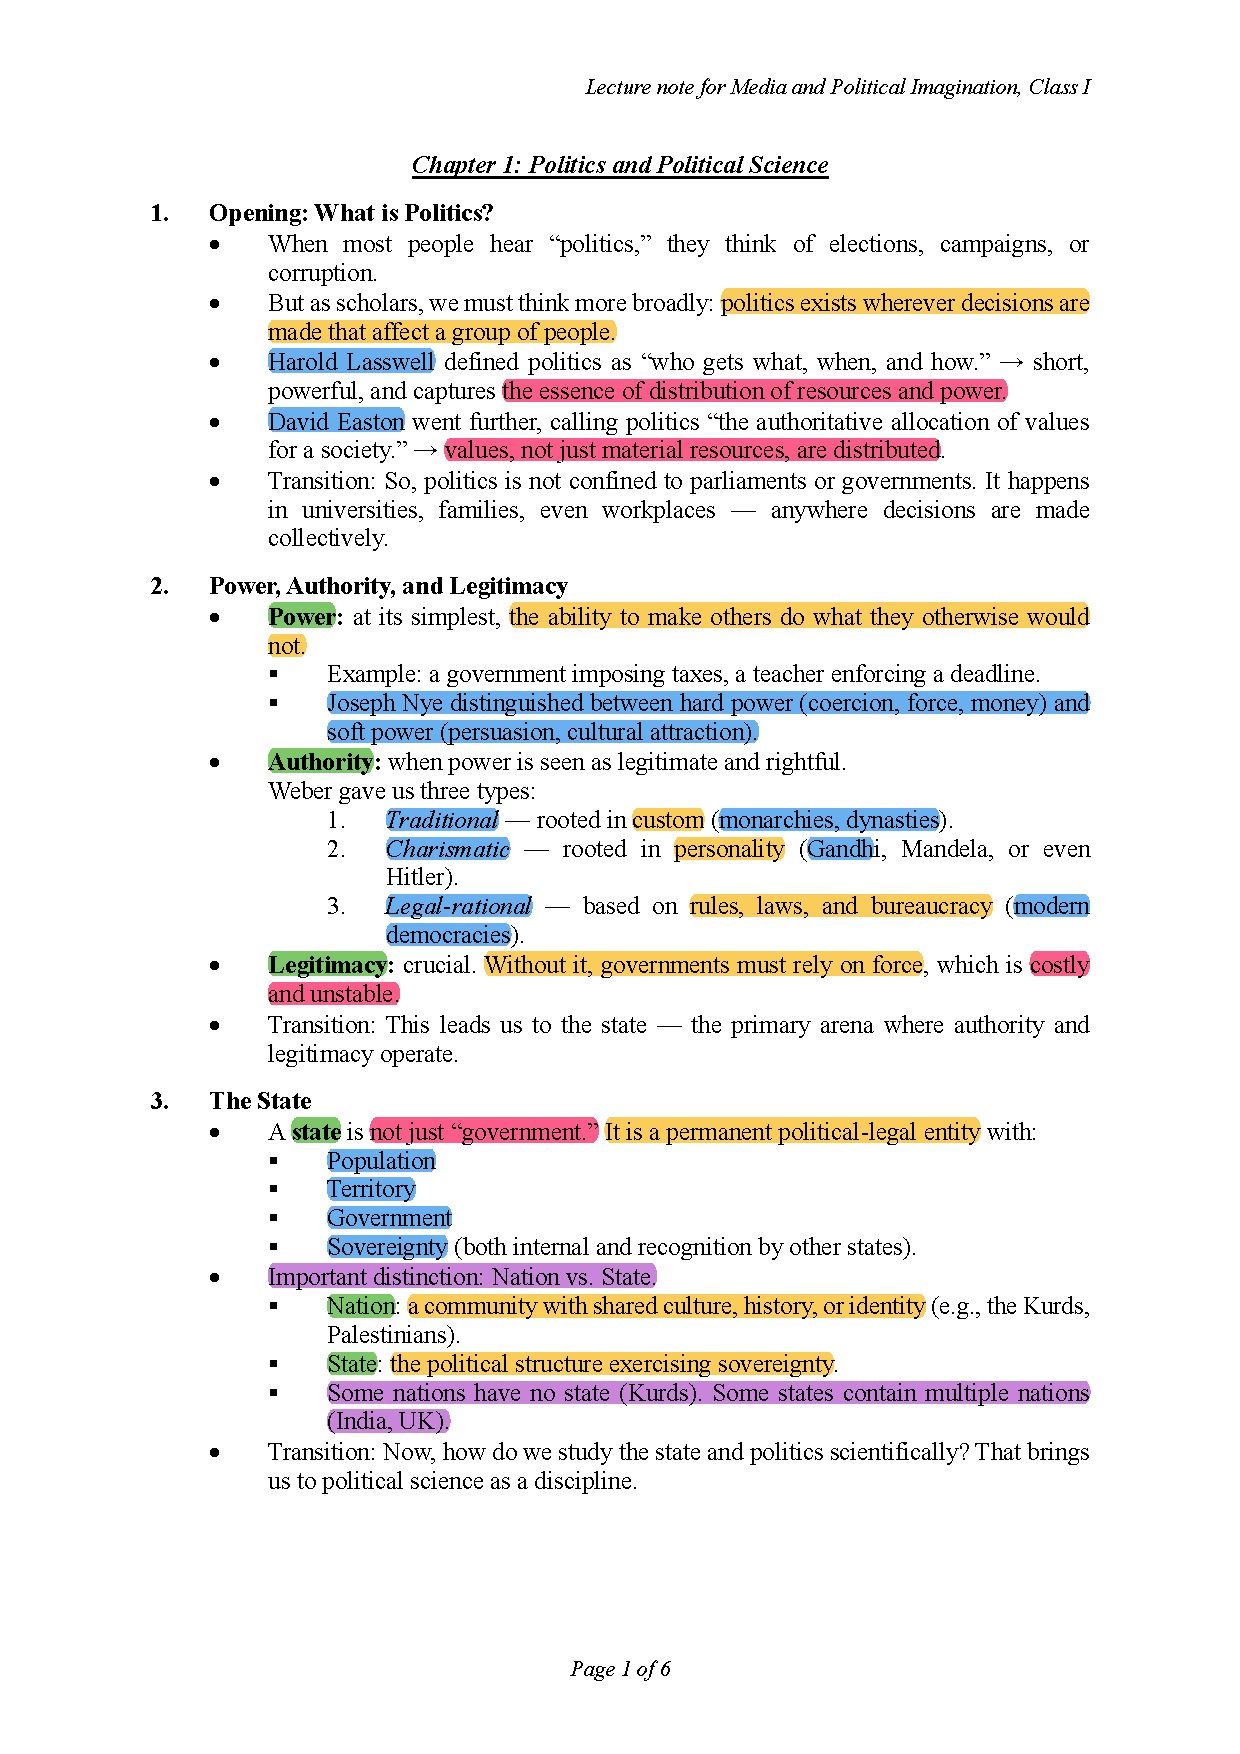
\includepdf[page=-]{Materials/Lecture_note_for_MPI_class_one.pdf}
				
				\textbf{What the FUCK is politics?}
				
				\begin{itemize}
					\item As scholars, we must think that politics exists where ever decisions are made that affect a group of people.
					\item Harold Lasswell defined politics as \textquotedblleft
				\end{itemize}
				
				\subsection{Power, Authority, and Legitimacy}
				
				\begin{itemize}
					\item Power is the simplest ability to make others do what they otherwise would not.
						\begin{itemize}
							\item Example: a government imposing taxes, a teacher enforcing a deadline.
							\item Joseph Nye distinguished between hard power (coercion, force, money) \& soft power (persuasion, cultural attraction)
						\end{itemize}
				\item Authority: when power is seen as legitimate and rightful.
				
				Weber gave us three types:
						\begin{itemize}
							\item Traditional \textemdash \space rooted in custom (monarchies, dynasties).
							\item Charismatic \textemdash \space rooted in personality (\textit {Gandhi, Mandela, or \textbf{Hitler}})
							\item Legal-rational \textemdash \space based on rules, laws, and bureaucracy (modern democracy)
						\end{itemize} 
			
				\item Legitimacy: \textbf{crucial}. without it governments must rely on force, which is costly and unstable.
			\end{itemize}
			
			\subsection{The State}
			\begin{itemize}
				\item A state is not just a "government." It is a permanent political-legal entity with: 
					\begin{itemize} 		
					\item population
					\item territory
					\item government
					\item sovereignty (both internal and recognition by other states)
					\end{itemize}
				\item Important distinction: Nation vs State.
					\begin{itemize}
					\item Nation: a community with shared culture, history, or identity (e.g., The Kurds, Palestinians).
					\item State: the political structure exercising sovereignty.
					\end{itemize}	
			\end{itemize}
			
			\subsection{Political Science as a discipline}
			\begin{itemize}
				\item Originally, focusing on institution: constitution, parliaments, and courts
				\item Post-WWII, become more specific approach \textemdash \space behavioral revolution
					\begin{itemize}
						\item Political behavior: voting, protest, opinion surveys. 
					\end{itemize}
				\end{itemize}
			\begin{itemize}
				\item Today, political science spans:
				\begin{itemize} 
				\item Political theory and philosophy \textemdash what justice and democracy ought to be
				\item Comparative politics \textemdash how systems differ
				\item International relations \textemdash war, diplomacy, globalization
				\item Public policy and administration
				\end{itemize}
			\end{itemize}
			
		\subsection{Approaches in Political Science}
		\begin{itemize}
			\item Normative: ``what ought to be\textquotedblright
			\item Empirical: ``what is"
			\item Behavioralism (1950s-60s): adopted psychology and statistics; highlighted observable behavior.
			\item Post-behavioralism (1970s): behavioralism’s cold empiricism sparked a demand for research relevant to human problems.
		
		\end{itemize}
		
		
		
		
						
\part{Course Summary.}
	\chapter{Topic}

\end{document}
